\DiaryEntry{Groups and GAP, II}{2023-06-05}{Algebra}

We started in \ref{2020-09-25:entry} with group theory using GAP; here we continue by additional examples.

\subsection{Dihedral Groups}

\paragraph{Basics.} We have covered Dihedral groups in entry \ref{2023-06-13:entry}. A Diheadral group $D_n$ is defined as all products of the two elements $r$ and $s$ which satisfy the following conditions:

\begin{align*}
r^n &= 1 \\
s^2 &= 1 \\
srs &= r^{-1}
\end{align*}

Gap has a predefined Dihedral group which is created by \verb+DihedralGroup(n);+. We can create the group and define $r$ and $s$ as follows.

\begin{verbatim}
    gap> TeachingMode(true);
    #I  Teaching mode is turned ON
    gap> D8:=DihedralGroup(8);
    <fp group of size 8 on the generators [ r, s ]>
    gap> e:=Elements(D8);
    [ <identity ...>, r^-1, r, s, r^2, r*s, s*r, s*r^2 ]
    gap> r:=e[3];
    r
    gap> s:=e[4];
    s
\end{verbatim}

This matches the definition from above as we find

\begin{verbatim}
    gap> r^2;
    r^2
    gap> r^3;
    r^-1
    gap> r^4;
    <identity ...>
    gap> s^2;
    <identity ...>
\end{verbatim}

We can also display the relators (ie the set of defining equations) of the group,

\begin{verbatim}
	gap> RelatorsOfFpGroup(DihedralGroup(8));
	[ r^4, s^2, s^-1*r*s*r ]
\end{verbatim}

The first two exactely follow our definition; for the last we have $s^{-1}rsr = e \rightarrow rsr = s \rightarrow sr = r^{-1}s \rightarrow srs = r^{-1}ss = r^{-1}$. \qed


We can obtain the main properties for $D_8$,

\begin{verbatim}
    gap> IsAbelian(D8);
    false
    gap> IsCyclic(D8);
    false
    gap> Order(D8);
    8
\end{verbatim}

From the \href{https://nathancarter.github.io/group-explorer/Multtable.html?groupURL=https://nathancarter.github.io/group-explorer/groups/D_4.group}{Group Explorer} we obtain the following multiplication table for $D_4$. Note that the table uses $f$ instead of $s$ and uses a different definition of $n$!

\begin{figure}[H]
    \centering
    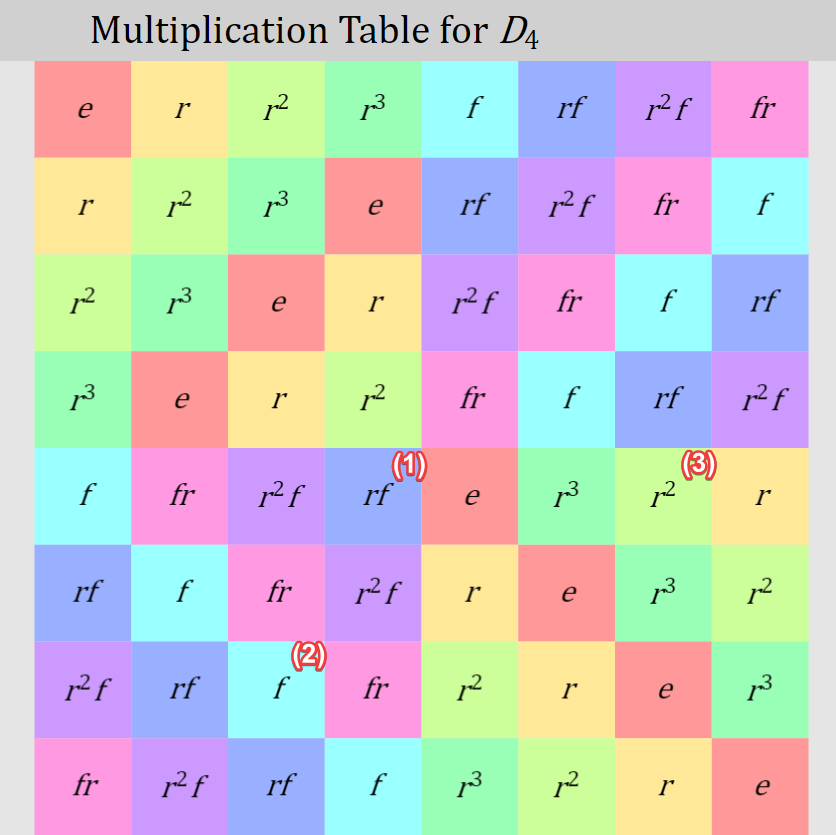
\includegraphics[scale=0.35]{images/2023-06-05_groups_gap_D4.png}
\end{figure}

We can compare some cases with Gap (the numbers in the Figure corresponds to the numbers in the session below)

\begin{verbatim}
    gap> s*r^3;     # item (1)
    r*s
    gap> r^2*s*r^2; # item (2)
    s
    gap> s*r^2*s;   # item (3)
    r^2
\end{verbatim}

When we store the elements of the group in a variable \verb+e+, and store the number of elements in \verb+n+, then we can produce the multiplication table via Gap (slightly edited for readability).

\begin{verbatim}
    gap> e:=Elements(D8);
    [ <identity ...>, r^-1, r, s, r^2, r*s, s*r, s*r^2 ]
    gap> n:=Size(e);
    8
    gap> M:=MultiplicationTable(D8);
    [ [ 1, 2, 3, 4, 5, 6, 7, 8 ], [ 2, 5, 1, 7, 3, 4, 8, 6 ], 
	  [ 3, 1, 5, 6, 2, 8, 4, 7 ], [ 4, 6, 7, 1, 8, 2, 3, 5 ], 
      [ 5, 3, 2, 8, 1, 7, 6, 4 ], [ 6, 8, 4, 3, 7, 1, 5, 2 ], 
	  [ 7, 4, 8, 2, 6, 5, 1, 3 ], [ 8, 7, 6, 5, 4, 3, 2, 1 ] ]
    gap> for i in [1..n] do
    >         for j in [1..n] do
    >         ind := M[i][j];
    >         Print(e[ind], "   ");
    >         od;
    >     Print("\n");
    >     od;

    e     r^-1   r      s      r^2   r*s    s*r    s*r^2   
    r^-1  r^2    e      s*r    r     s      s*r^2  r*s   
    r     e      r^2    r*s    r^-1  s*r^2  s      s*r   
    s     r*s    s*r    e      s*r^2 r^-1   r      r^2   
    r^2   r      r^-1   s*r^2  e     s*r    r*s    s   
    r*s   s*r^2  s      r      s*r    e     r^2    r^-1   
    s*r   s      s*r^2  r^-1   r*s   r^2    e      r   
    s*r^2 s*r    r*s    r^2    s     r      r^-1   e   
\end{verbatim}

The ordering of the columns is different compared to GroupExplorer; in addition, Gap seems to minimize the exponents (at the expense of negative ones); eg prefering \verb+r^-1 + over \verb+r^3+. Therefore, the result looks different than the table from GroupExplorer, but contains the same information.

\paragraph{Permutation Representation.} We can also get the group elements as permutations (that makes interpretation in terms of how the element affect points easier),

\begin{verbatim}
    gap> DihedralGroup(IsPermGroup, 8);
    Group([ (1,2,3,4), (2,4) ])
    gap> e:=Elements(DihedralGroup(IsPermGroup, 8));
    [ (), (2,4), (1,2)(3,4), (1,2,3,4), (1,3), (1,3)(2,4), 
	  (1,4,3,2), (1,4)(2,3) ]
\end{verbatim}

If we consider a square with points labelled $1, 2, 3, 4$ as shown below, the Dihedral Group $D_4$ contains the following:

\begin{itemize}
    \item The identity element, doing nothing
    \item Two reflections along the horizonal and vertical axis exchanging 4 points each: The horizontal one exchanges point $1$ with $4$ and point $2$ with $3$; this corresponds to the permutation $(1,4)(2,3)$. The other one is vertical, exchanges point $1$ with $2$ and point $3$ with point $4$; this corresponds to $(1,2)(3,4)$.
    \item Two reflections along diagonals, each exchanging only two points: One exchanges point $2$ with point $4$, corresponding to $(2,4)$, the other exchanges point $1$ with point $3$, corresponding to $(1,3)$.
    \item A combined reflection $(1,3)(2,4)$.
    \item Two rotations; one clockwise corresponding to $(1,2,3,4)$, the other counter-clockwise corresponding to $(1,4,3,2)$.
\end{itemize}


\begin{figure}[H]
    \centering
    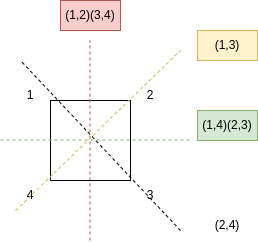
\includegraphics[scale=0.75]{images/2023-06-05_groups_gap_D4_2.png}
\end{figure}

We can display the mapping from permutations to "equation symbols" as follows.

\begin{verbatim}
	gap> GroupHomomorphismByImages(DihedralGroup(IsPermGroup, 8), DihedralGroup(8));
	[ (1,2,3,4), (2,4) ] -> [ r, s ]
\end{verbatim}

With this knowledge, we can (manually) create a mapping table from "equation symbols" to permutations.

\begin{verbatim}
r^-1 -> (1,4,3,2)
r    -> (1,2,3,4)
s    -> (2,4)
r^2  -> (1,3(2,4)
rs   -> (1,4(2,3)
sr   -> (1,2)(3,4)
sr^2 -> (1,3)
\end{verbatim}

The order of the group elements are as follows,

\begin{verbatim}
    for x in DihedralGroup(IsPermGroup, 8) do
        Print(x, " has order ", Order(x), "\n");
    od;
    () has order 1
    (2,4) has order 2
    (1,3)(2,4) has order 2
    (1,3) has order 2
    (1,4,3,2) has order 4
    (1,4)(2,3) has order 2
    (1,2,3,4) has order 4
    (1,2)(3,4) has order 2
\end{verbatim}

Since every group can be expressed as subgroup of the Symmetric Group, we can also define the Dihedral Group this way. We start by displaying all subgroups of $S_4$ in the hope to find the subgroup expressed as above as 
\verb+Group([ (1,2,3,4), (2,4) ])+. Unfortunately, this is not the case. So we ask Gap for a group description
(\verb+StructureDescription+) and work backwards to identify $D_4$.

\begin{Verbatim}[commandchars=\\\{\}]
    gap> sg:=AllSubgroups(SymmetricGroup(4));
    [ Group(()), Group([ (1,2)(3,4) ]), Group([ (1,3)(2,4) ]), 
    Group([ (1,4)(2,3) ]), Group([ (3,4) ]), Group([ (2,3) ]), 
    Group([ (2,4) ]), Group([ (1,2) ]), Group([ (1,3) ]), 
    Group([ (1,4) ]), Group([ (2,4,3) ]), Group([ (1,3,2) ]), 
    Group([ (1,4,2) ]), Group([ (1,4,3) ]), Group([ (1,4)(2,3), (1,3)(2,4) ]),
    Group([ (3,4), (1,2)(3,4) ]), Group([ (1,4), (1,4)(2,3) ]), 
    Group([ (2,4), (1,3)(2,4) ]), Group([ (1,3,2,4), (1,2)(3,4) ]),
    Group([ (1,4,3,2), (1,3)(2,4) ]), Group([ (1,2,4,3), (1,4)(2,3) ]), 
    Group([ (3,4), (2,4,3) ]), Group([ (1,4), (1,4,3) ]), 
    Group([ (2,3), (1,3,2) ]), Group([ (1,2), (1,4,2) ]), 
    \textcolor{red}{Group([ (1,4)(2,3), (1,3)(2,4), (3,4) ])},
    \textcolor{red}{Group([ (1,2)(3,4), (1,3)(2,4), (1,4) ])},
    \textcolor{red}{Group([ (1,2)(3,4), (1,4)(2,3), (2,4) ])},
    Group([ (1,4)(2,3), (1,3)(2,4), (2,4,3) ]), 
    Group([ (1,4)(2,3), (1,3)(2,4), (2,4,3), (3,4) ]) ]
    gap> List(sg, StructureDescription);
    [ "1", "C2", "C2", "C2", "C2", "C2", "C2", "C2", "C2", "C2", 
      "C3", "C3", "C3", "C3", "C2 x C2", "C2 x C2", "C2 x C2", 
      "C2 x C2", "C4", "C4", "C4", "S3", "S3", "S3", "S3", 
      \textcolor{red}{"D8", "D8", "D8"}, "A4", "S4" ]
\end{Verbatim}

Above subgroups labelled as $D_8$ have different generators than what Gap returned (\verb+Group([ (1,2,3,4), (2,4) ])+); nevertheless, we are almost there; in the third group (\verb+Group([ (1,2)(3,4), (1,4)(2,3), (2,4) ])+), let's define

\begin{verbatim}
    gap> g1:=(1,2)(3,4);;
    gap> g2:=(1,4)(2,3);;
    gap> g3:=(2,4);;
\end{verbatim}

and then we have

\begin{verbatim}
    gap> g2*g3;
    (1,2,3,4)
\end{verbatim}

\qed.

\paragraph{Description as Free Group.} We can define a free group in Gap and assign the three defining characteristics of $D_4$ (namely $r^4 = 1, s^2 = 1, srs = r^{-1} \rightarrow rsrs = 1$) to the group.

\begin{verbatim}
    gap> f := FreeGroup("r", "s");;
    gap> AssignGeneratorVariables(f);;
    #I  Assigned the global variables [ r, s ]
    gap> g:=f/[r^4, s^2, r*s*r*s];
    <fp group on the generators [ r, s ]>
    gap> StructureDescription(g);
    "D8"
    gap> Elements(g);
    [ <identity ...>, r, s, r^2, r*s, r^-1, r^2*s, r^-1*s ]
\end{verbatim}

\subsection{Free Groups}

We can pick up the previous description form and work with free groups. With \\ \verb+FreeGroup("a", "b")+ we can define a free group with generators $a$ and $b$. The command \verb+AssignGeneratorVariables(f)+ creates corresponding variables $a$ and $b$ in Gap. We then define a subgroup by stating the equations for the unity element $e$; in the example below, we use the equations for the symmetric group $S_3$, $a^3 = b^2 = e, bab = a^{-1}$. Rewriting the last equation as $abab=e$, we obtain in Gap,

\begin{verbatim}
    gap> f := FreeGroup("a", "b");;
    gap> AssignGeneratorVariables(f);;
    #I  Assigned the global variables [ a, b ]
    gap> g:=f/[a^3, b^2, a*b*a*b];
    <fp group on the generators [ a, b ]>
    gap> StructureDescription(g);
    "S3"
    gap> Order(g);
    6
    gap> Elements(g);
    [ <identity ...>, b, a, a^-1*b, a^-1, a*b ]
\end{verbatim}

This raises the questions whether there are groups of order $6$ having a different structure. This can be answered by Gap's SmallGroup Library which is basically a large database of groups.

\begin{verbatim}
    gap> SmallGroupsInformation(6);

    There are 2 groups of order 6.

    The groups whose order factorises in at most 3 primes 
    have been classified by O. Hoelder. This classification is 
    used in the SmallGroups library. 

    This size belongs to layer 1 of the SmallGroups library. 
    IdSmallGroup is available for this size. 
\end{verbatim}

We can retrieve the groups from the library and obtain further information about them.

\begin{verbatim}
    gap> g1:=SmallGroup(6,1);
    <pc group of size 6 with 2 generators>
    gap> StructureDescription(g1);
    "S3"
    gap> g2:=SmallGroup(6,2);
    <pc group of size 6 with 2 generators>
    gap> StructureDescription(g2);
    "C6"
\end{verbatim}

The two groups are $S_3$ and $C_6$; this matches with the results in the GroupExplorer. What is weird is the following.

\begin{verbatim}
    gap> Elements(g2);
    [ <identity> of ..., f1, f2, f1*f2, f2^2, f1*f2^2 ]
    gap> M:=MultiplicationTable(g2);
    [ [ 1, 2, 3, 4, 5, 6 ], [ 2, 1, 4, 3, 6, 5 ], [ 3, 4, 5, 6, 1, 2 ], 
      [ 4, 3, 6, 5, 2, 1 ], [ 5, 6, 1, 2, 3, 4 ], [ 6, 5, 2, 1, 4, 3 ] ]
\end{verbatim}

The multiplication table of the cyclic group $C_6$ is really different and I don't know if the two are equivalent...

\begin{verbatim}
    gap> MultiplicationTable(CyclicGroup(6));
    [ [ 1, 2, 3, 4, 5, 6 ], [ 2, 3, 4, 5, 6, 1 ], [ 3, 4, 5, 6, 1, 2 ], 
      [ 4, 5, 6, 1, 2, 3 ], [ 5, 6, 1, 2, 3, 4 ], [ 6, 1, 2, 3, 4, 5 ] ]
\end{verbatim}

We can use some Gap magic to find out whether two groups are isomorphic or not \todo{add citation!}

\begin{verbatim}
gap> AreIsomorphic := function(G, H)
> return not IsomorphismGroups(G, H) = fail;
> end;
function( G, H ) ... end
gap> AreIsomorphic(g2, CyclicGroup(6));
true
\end{verbatim}

So, yes, the two groups are isomorphic! Let's work out how the isommorphism looks like using Gap. We can use the function \verb+IsomorphismGroups+,

\begin{verbatim}
gap> IsomorphismGroups(s2, C6);
[ f1, f2^2 ] -> [ a^3, a^2 ]
\end{verbatim}


The elements of \verb+g2+ are \verb+e, f1, f2, f1*f2, f2^2, f1*f2^2 + (see further above). Using the isommorphism provided by Gap, we can rewrite this as \\
\verb+e, a^3, f2, f1*f2, a^2, a^5+; the mapping of two elements is still open (\verb+f2+ could be either \verb+a+ or \verb+a^4 +).

Let's assume that \verb+f2 = a^4 +. From the group structure we know that $a^6 = e$ and therefore \verb+f2 f2^2 = e+. Let's check in Gap (using the fact that \verb+e[5] = a^2+ ),

\begin{verbatim}
gap> e[3]*e[5];
<identity> of ...
\end{verbatim}

which confirms our assumption. The element \verb+f1*f2+ now becomes \verb+a^5 + and the elements of the group \verb+g2+ are \verb+e, a^3, a^4, a, a^2, a^5+ .


%%% Local Variables:
%%% mode: latex
%%% TeX-master: "journal"
%%% End:
